\section{从正定核构造空间}
\label{sec:rkhs-from-kernel}

上一节从空间出发得到核，并发现核的Gram矩阵总是半正定的。实际问题中往往反过来：人们先写下一个衡量两点相似程度的二元函数，再问它对应什么样的函数空间。

有限维中这个问题的答案已经知道。给定对称正定矩阵$\bm K$，令$\bm A=\bm K^{-1}$，就得到以$\bm K$为读坐标矩阵的内积空间。无限维中$\bm A$通常不存在，所以构造必须只用$\bm K$本身。本节证明，只要二元函数满足有限点组上的半正定条件，就存在唯一的RKHS以它为再生核。

构造分三步：先在核截面的有限线性组合上定义内积，并检查它不依赖于组合的写法；再处理长度为零的方向；最后完备化，并确认补进来的极限元素仍然是函数。

\subsection{正定核}
\label{sec:rkhs-pd-kernels}

定理~\ref{thm:rkhs-kernel-properties}的第1、2条只涉及核在有限个点上的值。把它们单独拿出来，就得到对二元函数的要求：把$K$看成下标取遍$X\times X$的矩阵，要求它的每个有限子矩阵都半正定。

\begin{definition}[正定核与严格正定核]
\label{def:rkhs-pd-kernel}
设$X$是非空集合，$K:X\times X\to\mathbb K$。若对任意$n\geq1$、任意点$x_1,\ldots,x_n\in X$与任意$c_1,\ldots,c_n\in\mathbb K$，
\begin{equation}
\sum_{i,j=1}^n\overline{c_i}\,c_j\,K(x_i,x_j)\geq0 ,
\label{eq:rkhs-pd-condition}
\end{equation}
并且在$\mathbb K=\mathbb R$时还有$K(x,y)=K(y,x)$，则称$K$为$X$上的\term{正定核}（positive definite kernel）。若进一步对任意\emph{互异}的点$x_1,\ldots,x_n$及不全为零的系数，上式严格大于零，则称$K$为\term{严格正定核}（strictly positive definite kernel）。
\end{definition}

用矩阵的语言，正定核要求每个Gram矩阵$\bm G=[K(x_i,x_j)]_{i,j}$都是Hermite半正定矩阵，严格正定核要求互异点组上的Gram矩阵都是正定矩阵，因而可逆。在复数情形，二次型对一切复系数取实值已经迫使$\bm G$是Hermite矩阵，所以不必另加对称条件；实数情形只用实系数检验，对称性必须单独要求。

“正定核”是通行的名称，但它只要求Gram矩阵\emph{半}正定，允许矩阵奇异。之所以要区分严格正定，是因为后文有限观测问题能否对任意数据求解，正取决于Gram矩阵是否可逆。定义中强调互异的点：若$x_1=x_2$，Gram矩阵的前两行相同，任何核的这个矩阵都奇异。

\paragraph{半正定但不严格正定的例子}

仿射核$K(x,y)=1+xy$由上一节的空间得到，所以是正定核。取三个互异点$-1,0,1$，Gram矩阵及其一个零向量为
\[
\bm G=\begin{bmatrix}2&1&0\\1&1&1\\0&1&2\end{bmatrix},\qquad
\bm G\begin{bmatrix}1\\-2\\1\end{bmatrix}=\bm 0 .
\]
对应的函数组合恰好是零函数：
\[
K_{-1}-2K_0+K_1=(1-t)-2+(1+t)=0 .
\]
原因是$H_{\mathrm{aff}}$只有二维，任意三个核截面必然线性相关。所以仿射核正定而不严格正定。

\paragraph{严格正定的例子}

\term{高斯核}（Gaussian kernel）是最常用的严格正定核：
\[
K_\sigma(x,y)=\exp\Bigl(-\frac{\lvert x-y\rvert^2}{2\sigma^2}\Bigr)\qquad(x,y\in\mathbb R).
\]
它的严格正定性可以直接证明。第~\ref{chap:fourier-transform}章算过Gauss函数的Fourier变换，把那里的结果作伸缩，下式对一切实数$u$成立：
\[
\exp\Bigl(-\frac{u^2}{2\sigma^2}\Bigr)=\int_{\mathbb R}\mathrm e^{\mathrm i\omega u}\,p_\sigma(\omega)\,\mathrm d\omega,\qquad
p_\sigma(\omega)=\frac{\sigma}{\sqrt{2\pi}}\mathrm e^{-\sigma^2\omega^2/2}.
\]

取互异的$x_1,\ldots,x_n$与系数$c_j$，令
\[
g(\omega)=\sum_jc_j\mathrm e^{-\mathrm i\omega x_j}.
\]
把$u=x_i-x_j$代入二次型，交换有限和与积分，被积函数恰好成为一个模平方：
\[
\sum_{i,j}\overline{c_i}\,c_j\,K_\sigma(x_i,x_j)=\int_{\mathbb R}\lvert g(\omega)\rvert^2\,p_\sigma(\omega)\,\mathrm d\omega\geq0 .
\]

若积分为零，由$p_\sigma>0$与$g$连续，$g$恒为零。对$g$在$\omega=0$处求$k$阶导数，$k=0,\ldots,n-1$，得到
\[
\sum_{j=1}^nc_j\,x_j^k=0 .
\]
这是系数矩阵为Vandermonde矩阵的齐次方程组，点互异时只有零解，所以$c_1=\cdots=c_n=0$。这就证明了高斯核严格正定。

在两个点$0,1$、$\sigma=1$上可以直接核对：Gram矩阵及其特征值为
\[
\begin{bmatrix}1&\mathrm e^{-1/2}\\\mathrm e^{-1/2}&1\end{bmatrix},\qquad
1\pm\mathrm e^{-1/2}\approx1.607,\ 0.393,
\]
两个特征值都为正。

图~\ref{fig:rkhs-gram-matrices}在五个点上比较这两种核。两者都是半正定矩阵，高斯核的五个特征值都为正，仿射核只有两个正特征值，其余为零。这幅图只检验了一个点组，严格正定性需要像上面那样对一切互异点组论证。

\begin{BookInlineFigure}
  \centering
  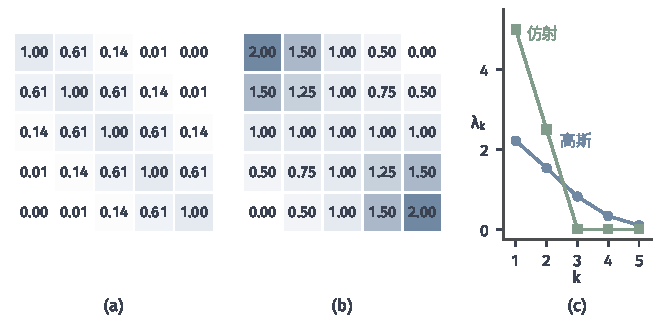
\includegraphics[width=112mm]{figures/04-spaces-measures-and-geometry/03-function-spaces/matplotlib/rkhs-gram-matrices/figure.pdf}
  \caption{点组$x=-1,-0.5,0,0.5,1$上的Gram矩阵。(a)高斯核（$\sigma=0.5$），颜色越深核值越大，数字保留两位小数（右上角的$0.00$实为$\mathrm e^{-8}\approx0.0003$）。(b)仿射核$1+xz$。(c)两个矩阵的特征值从大到小排列：高斯核为$2.217,1.531,0.820,0.333,0.099$，全为正；仿射核只有$5$与$2.5$两个正特征值。两种核都半正定，只有前者的矩阵可逆。}
  \label{fig:rkhs-gram-matrices}
\end{BookInlineFigure}

\subsection{核截面的有限线性组合}
\label{sec:rkhs-finite-combinations}

下面固定$X$上的一个正定核$K$。如果以$K$为再生核的空间存在，它必定含有全部核截面$K_x=K(\cdot,x)$，并且由式~\eqref{eq:rkhs-kernel-definition}，截面之间的内积只能是$\langle K_x,K_y\rangle=K(x,y)$。构造就从这两点出发。

\paragraph{有限维的样板：只用$\bm K$写内积}

先在有限维中看怎样不用逆矩阵写出内积。矩阵$\bm K$的列的线性组合形如$\bm K\bm c$。若$\bm K$可逆，把$\bm K\bm c$与$\bm K\bm d$代入内积，逆矩阵$\bm A$被消掉：
\[
\langle\bm K\bm c,\bm K\bm d\rangle_{\bm A}=\bm c^{\top}\bm K\bm A\bm K\bm d=\bm c^{\top}\bm K\bm d .
\]
最右端只含$\bm K$，$\bm K$奇异时照样有意义。这时同一个向量可以由不同的系数表示，$\bm K$的零向量就是长度为零的系数方向。下面的构造逐字重复这个想法。

\paragraph{半内积}

令$H_0=\operatorname{span}\{K_x:x\in X\}$，它的元素是有限和，也就是$X$上的函数：
\[
f=\sum_ia_iK_{x_i},\qquad f(t)=\sum_ia_iK(t,x_i).
\]
对这样的$f$与另一个元素$g=\sum_jb_jK_{y_j}$，按上述要求规定
\begin{equation}
\langle f,g\rangle_0=\sum_{i,j}\overline{a_i}\,b_j\,K(x_i,y_j).
\label{eq:rkhs-h0-inner}
\end{equation}
它对$g$线性、对$f$共轭线性，具有共轭对称性，并且由正定条件知$\langle f,f\rangle_0\geq0$。

问题在于，同一个函数可以有多种有限和表示，例如仿射核下$K_{-1}+K_1$与$2K_0$是同一个函数。必须先检查式~\eqref{eq:rkhs-h0-inner}的值不依赖于表示的选取。

固定$i$先对$j$求和，因为$g(x_i)=\sum_jb_jK(x_i,y_j)$，得到第一种写法。固定$j$先对$i$求和，并用$K(x_i,y_j)=\overline{K(y_j,x_i)}$，得到第二种写法：
\[
\langle f,g\rangle_0=\sum_i\overline{a_i}\,g(x_i)
=\sum_jb_j\,\overline{f(y_j)} .
\]
第一种写法只通过$g$的函数值依赖于$g$，第二种只通过$f$的函数值依赖于$f$。所以换掉$g$的表示不改变第一种写法，换掉$f$的表示不改变第二种写法，$\langle f,g\rangle_0$确实是两个\emph{函数}的量。

取$f=K_x$，第一种写法给出
\begin{equation}
\langle K_x,g\rangle_0=g(x)\qquad(g\in H_0),
\label{eq:rkhs-h0-reproducing}
\end{equation}
即再生性质在$H_0$上已经成立。

\paragraph{零范数方向的商}

现在看长度为零的方向。若把系数本身当作对象，即考虑有限支撑的系数族$a=(a_x)_{x\in X}$组成的线性空间$V$，并用式~\eqref{eq:rkhs-h0-inner}的右端定义$\langle a,b\rangle_V$，那么这只是一个半内积。仿射核的例子中，点$-1,0,1$上的系数$(1,-2,1)$非零，长度却为零。于是$\lVert a\rVert_V=\langle a,a\rangle_V^{1/2}$只是半范数，$d(a,b)=\lVert a-b\rVert_V$只是伪度量。

第~\ref{chap:metric-spaces}章对伪度量的处理是把零距离的点视为同一个点，作商空间。这里同样令
\[
N=\{a\in V:\lVert a\rVert_V=0\}.
\]
半内积的Cauchy--Schwarz不等式的证明只用到半正定性与线性，因此照样成立：
\[
\lvert\langle a,b\rangle_V\rvert\leq\lVert a\rVert_V\lVert b\rVert_V .
\]
由它可知，$a\in N$当且仅当$\langle a,b\rangle_V=0$对一切$b$成立，从而$N$是线性子空间，半内积下降到商空间$V/N$上成为真正的内积。

剩下的是把商空间与函数空间$H_0$对应起来。把系数$a$映为函数$f_a=\sum_xa_xK_x$，这个映射从$V$到$H_0$满射。记$e_t\in V$为只在$t$处取$1$、其余处取$0$的系数，则
\[
\langle e_t,a\rangle_V=\sum_xa_xK(t,x)=f_a(t),\qquad \lVert e_t\rVert_V^2=K(t,t).
\]
由半内积的Cauchy--Schwarz不等式，
\begin{equation}
\lvert f_a(t)\rvert=\lvert\langle e_t,a\rangle_V\rvert\leq\sqrt{K(t,t)}\,\lVert a\rVert_V .
\label{eq:rkhs-h0-point-bound}
\end{equation}

式~\eqref{eq:rkhs-h0-point-bound}说明，$a\in N$时$f_a$在每一点为零。反过来，$f_a\equiv0$时，
\[
\lVert a\rVert_V^2=\sum_x\overline{a_x}\,f_a(x)=0 .
\]
可见零范数的系数恰好是给出零函数的系数，商空间$V/N$与$H_0$一一对应，$\langle\cdot,\cdot\rangle_0$是$H_0$上真正的内积。把系数映成函数，恰好完成了零距离商。

\subsection{空间的完备化}
\label{sec:rkhs-completion}

$H_0$一般不完备。以最小值核为例，$H_0$由左端为零、在有限个节点处转折的连续折线组成，而下面这列折线的极限不是折线。取$m$个等距节点上核截面的平均：
\[
f_m=\frac1m\sum_{i=1}^mK_{i/m},\qquad K_{i/m}(t)=\min(t,\tfrac im).
\]
它的导数在第$k$段$(\tfrac{k-1}m,\tfrac km]$上等于$\tfrac{m-k+1}m$。

取$f(t)=t-t^2/2$，它的导数是$1-t$。在第$k$段上两个导数之差为$t-\tfrac{k-1}m$，所以
\[
\lVert f_m-f\rVert_{H_{\min}}^2=m\int_0^{1/m}u^2\,\mathrm du=\frac1{3m^2}.
\]
$(f_m)$在核范数下是Cauchy列，极限$t-t^2/2$属于$H_{\min}$，却不是折线，不在$H_0$中。下面补上这些极限，并确认它们仍然是$X$上的函数。

\paragraph{完备化与点值的极限}

由第~\ref{chap:metric-spaces}章，$H_0$有完备化$\overline{H_0}$，它由$H_0$中Cauchy列的等价类组成，$H_0$在其中稠密；内积沿Cauchy列取极限延拓过去，$\overline{H_0}$成为Hilbert空间。但完备化中的元素是抽象的等价类，还不是$X$上的函数，接下来要把它们变回函数。

点值估计~\eqref{eq:rkhs-h0-point-bound}正好提供这一步。若$(f_k)$是$H_0$中的Cauchy列，则
\[
\lvert f_k(x)-f_l(x)\rvert\leq\sqrt{K(x,x)}\,\lVert f_k-f_l\rVert_0 ,
\]
所以在每一点$f_k(x)$都是Cauchy数列，有确定的极限。两个等价的Cauchy列相差一列范数趋于零的函数，在每一点有相同的极限。用内积写出来，就是定义
\[
J:\overline{H_0}\to\mathbb K^X,\qquad (J\xi)(x)=\langle K_x,\xi\rangle_{\overline{H_0}} .
\]
若$f_k\to\xi$，则$f_k(x)=\langle K_x,f_k\rangle\to(J\xi)(x)$，所以$J\xi$就是逼近$\xi$的Cauchy列的逐点极限。由式~\eqref{eq:rkhs-h0-reproducing}，$J$在$H_0$上是恒等映射。

\paragraph{极限元素仍可识别为函数}

还剩一个危险：$\overline{H_0}$中两个不同的元素，会不会给出同一个函数？若是这样，函数之间就无法定义内积。等价地，要排除$\xi\neq0$而$J\xi$是零函数的情形。

若$\langle K_x,\xi\rangle=0$对一切$x$成立，则$\xi$与每个核截面正交，从而与它们的张成$H_0$正交。$H_0$在$\overline{H_0}$中稠密，所以$\xi$与整个空间正交，$\xi=0$。因此$J$是单射。

\begin{theorem}[由正定核确定再生核Hilbert空间]
\label{thm:rkhs-moore-aronszajn}
设$K$是非空集合$X$上的正定核。则存在唯一的RKHS，记为$H_K$，以$K$为其再生核。并且$H_0=\operatorname{span}\{K_x:x\in X\}$在$H_K$中稠密，$H_K$的每个元素都是$H_0$中某个Cauchy列的逐点极限。
\end{theorem}

\begin{proof}
先证存在性。令$H_K=J(\overline{H_0})$，规定
\[
\langle J\xi,J\eta\rangle_{H_K}=\langle\xi,\eta\rangle_{\overline{H_0}} .
\]
$J$是线性单射，这个定义良好，$J$成为等距同构，所以$H_K$是Hilbert空间；$J$的线性说明$H_K$中的加法和数乘就是逐点运算。

$J$在$H_0$上是恒等映射，故$K_x\in H_K$。对$f=J\xi$，由$J$的定义和等距性，
\[
f(x)=\langle K_x,\xi\rangle_{\overline{H_0}}=\langle JK_x,J\xi\rangle_{H_K}=\langle K_x,f\rangle_{H_K} .
\]
这就是以$K$为再生核的再生性质，点评估有界随之成立。稠密性与逐点极限的描述来自$H_0$在$\overline{H_0}$中稠密，以及上面关于$J$的讨论。

再证唯一性。设$H$是另一个以$K$为再生核的RKHS。$H$含有每个$K_x$，且$\langle K_x,K_y\rangle_H=K(x,y)$，所以$H_0\subseteq H$，两者在$H_0$上的内积一致。由定理~\ref{thm:rkhs-kernel-properties}的第4条，$H_0$在$H$中稠密。

任取$f\in H$及$H_0$中按$H$范数收敛到$f$的序列$f_k$。它是$H_0$中的Cauchy列，由再生性质逐点收敛到$f$。同一序列在$H_K$中收敛到其逐点极限，也就是$f$。所以$f\in H_K$，且
\[
\lVert f\rVert_{H_K}=\lim_k\lVert f_k\rVert_0=\lVert f\rVert_H .
\]
对调两个空间的角色，得$H=H_K$，再由极化恒等式知内积相同。
\end{proof}

这个结论通常称为Moore--Aronszajn定理\scite{aronszajn1950kernels}。图~\ref{fig:rkhs-construction-steps}用最小值核把构造的四个阶段画了出来。从此以后，“正定核”与“RKHS”可以互相确定：每个RKHS有唯一的再生核，每个正定核恰好是一个RKHS的再生核。

\begin{BookInlineFigure}
  \centering
  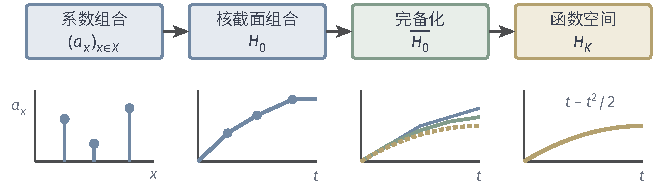
\includegraphics[width=111.1mm]{figures/04-spaces-measures-and-geometry/03-function-spaces/tikz/rkhs-construction-steps/figure.pdf}
  \caption{用最小值核走一遍由正定核构造$H_K$的四个阶段。第一栏是有限支撑的系数，二次型只给出半内积；第二栏把系数$(a_x)$变成函数$\sum_xa_xK_x$，这里是折线，零长度方向由此被商去；第三栏的蓝线、绿线是$m=2,4$时的平均折线$f_m$，虚线是它们在核范数下的极限；第四栏的$t-t^2/2$是该极限作为函数的样子，点值由Cauchy列逐点取极限得到。}
  \label{fig:rkhs-construction-steps}
\end{BookInlineFigure}

\paragraph{由最小值核重建$H_{\min}$}

以最小值核为例走一遍构造。核截面的导数是$\mathbf 1_{[0,x]}$，所以截面的内积可以写成导数的积分：
\[
\langle K_x,K_y\rangle_0=\min(x,y)=\int_0^1K_x'(t)\,K_y'(t)\,\mathrm dt .
\]
于是在$H_0$上$\lVert f\rVert_0=\lVert f'\rVert_{L^2}$。$H_0$中函数的导数恰好是区间上的阶梯函数，而阶梯函数在$L^2(0,1)$中稠密（第~\ref{chap:function-approximation}章）。于是完备化后的空间经由$f\mapsto f'$与$L^2(0,1)$等距同构，它就是上一节的$H_{\min}$。

这里唯一性起了作用：我们已经知道$H_{\min}$是以$\min(x,y)$为再生核的RKHS，定理~\ref{thm:rkhs-moore-aronszajn}保证从核出发构造的空间就是它，不必另作比较。

整个构造只用到集合$X$与核的正定性，没有用到测度或拓扑。所得的稠密性是在核范数意义下的，它不回答有限核截面组合能否逼近$H_K$之外的函数，这个问题留到第~\ref{sec:rkhs-section-span-approx}节。
